\localauthor{Thomas Kirz}

\subsection{Hochladen einer Revision}\label{subsec:sequenz-revision-hochladen}

Als Beispiel für einen Datenfluss wird in Abbildung~\ref{fig:upload-revision-sequence} ein Sequenzdiagramm zu folgendem Vorgang betrachtet:
Ein angemeldeter Nutzer ruft die Seite einer eigenen Einreichung auf, für die eine Revision angefordert wurde.
Dort fügt er eine Revision, also ein neues Paper hinzu.
Nach Erstellung der \code{UIMessage} wird ein Event gefeuert mit:
{\small
\begin{lstlisting}[language=Java]
    Event<UIMessage>#fire()
\end{lstlisting}
}
Dieses wird vom \code{UIMessageGenerator} observed, welcher dann eine \code{FacesMessage} hinzufügt,
die nach dem Hochladen auf der Einreichungsseite angezeigt wird.

\begin{figure}[H]
    \centering
    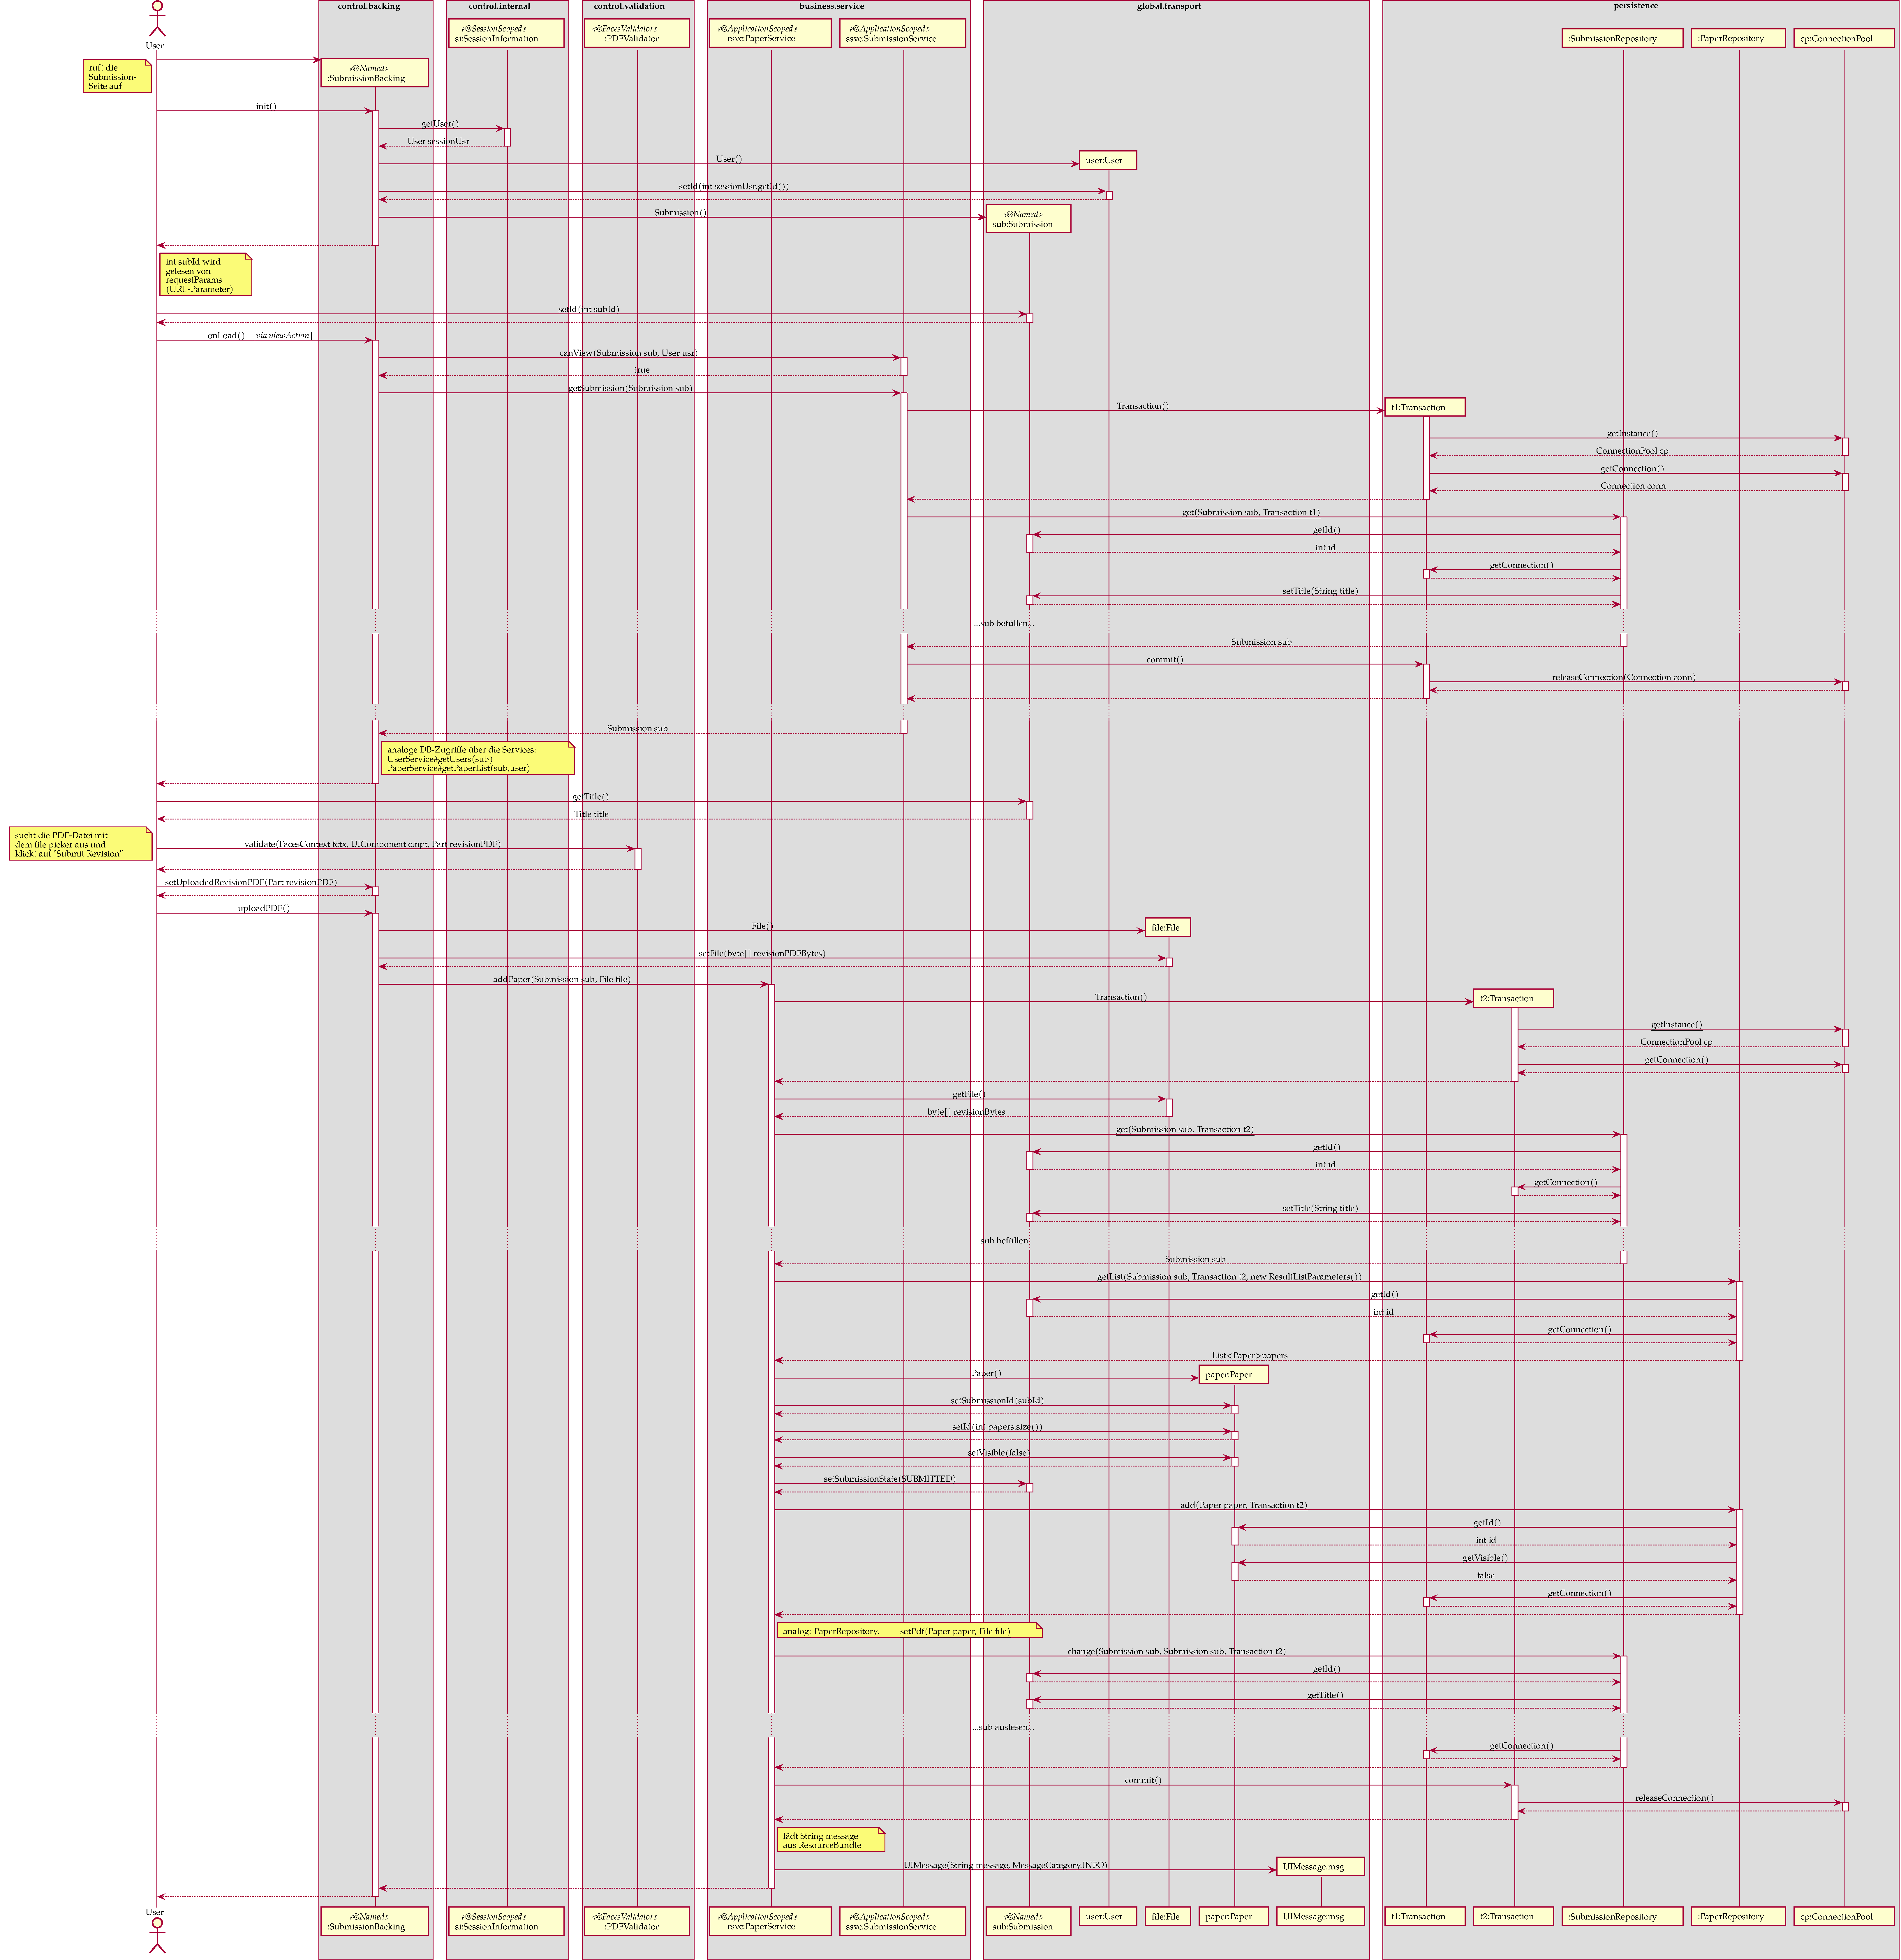
\includegraphics[width=0.9\textwidth]{graphics/upload_revision}
    \caption{Sequenzdiagramm zum Hochladen einer Revision}
    \label{fig:upload-revision-sequence}
\end{figure}

\subsection{Fehlerfall}\label{subsec:fehlerfall}

Abbildung~\ref{fig:upload-revision-sequence-failure} zeigt das gleiche Szenario wie Abbildung~\ref{fig:upload-revision-sequence},
jedoch passiert beim Datenbankzugriff für das Herunterladen der Einreichungsdaten ein Timeout.
Da dies ein fataler Fehler ist, wird der Nutzer mithilfe des \code{UncheckedExceptionHandlers} auf eine Fehlerseite weitergeleitet.

\begin{figure}[H]
    \centering
    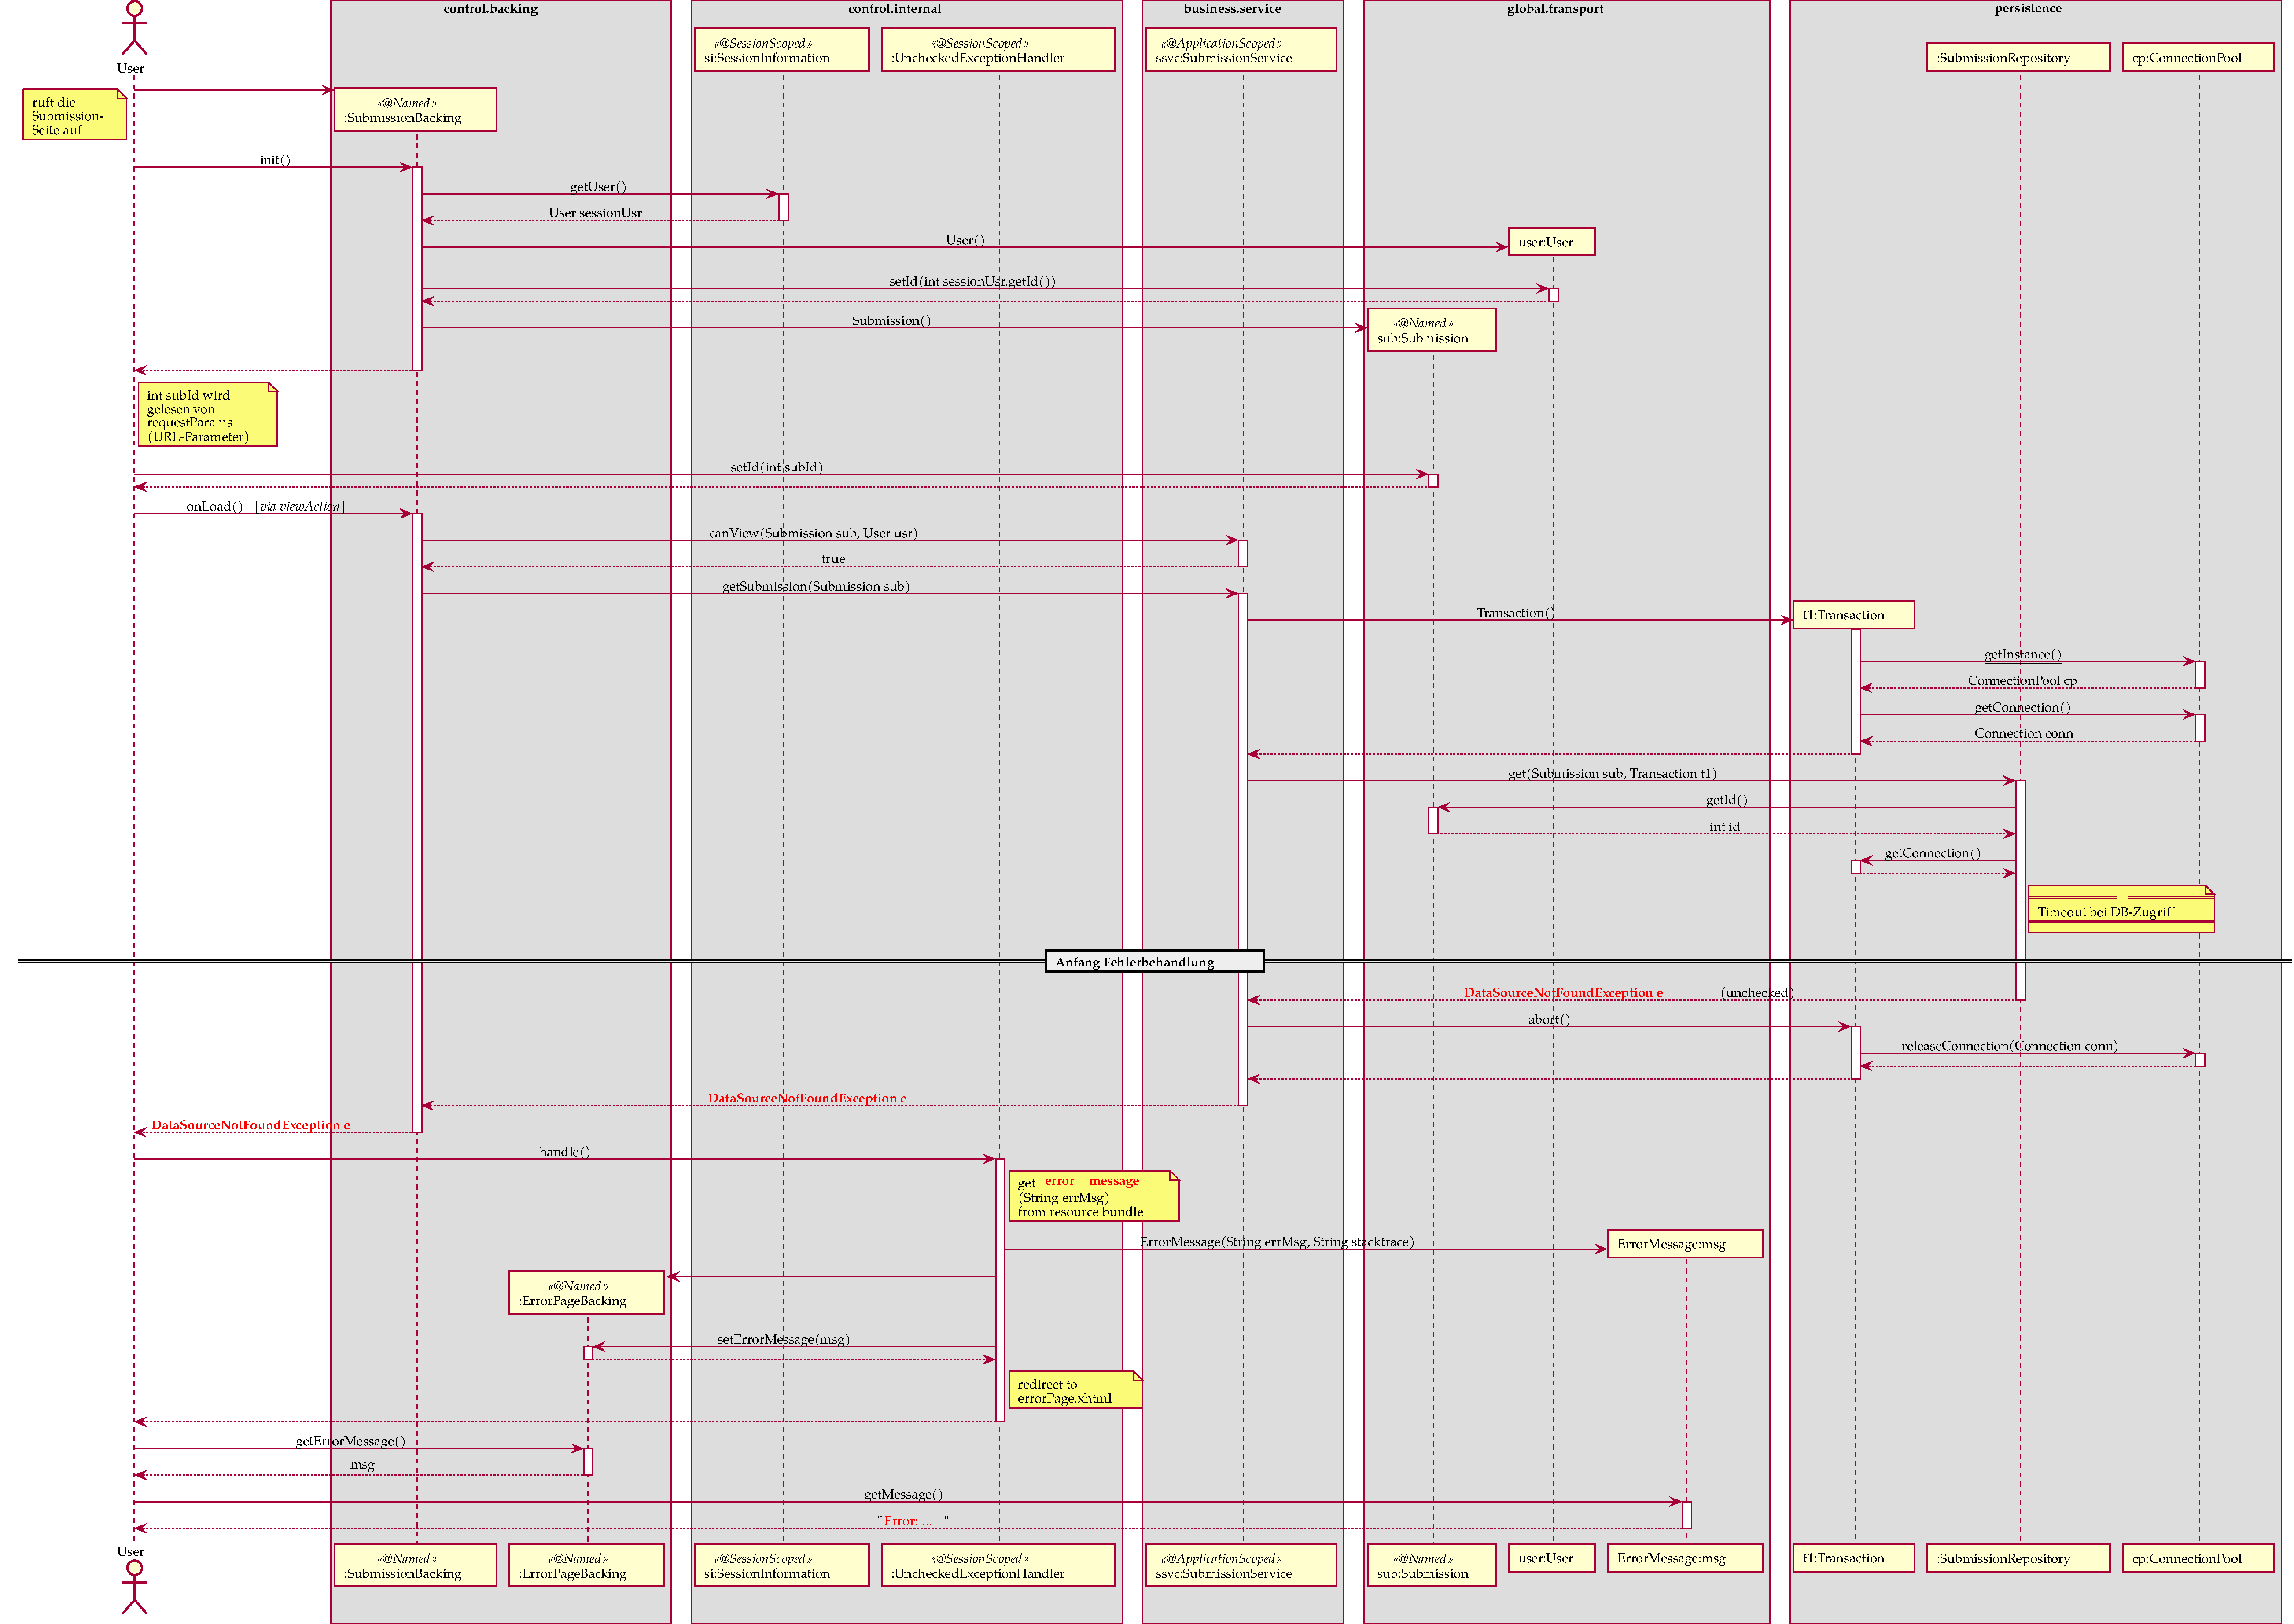
\includegraphics[width=0.9\textwidth]{graphics/upload_revision_failure}
    \caption{Sequenzdiagramm zum Aufruf einer Einreichungsseite mit Fehler beim Datenbankzugriff}
    \label{fig:upload-revision-sequence-failure}
\end{figure}
